\documentclass{beamer}

\usepackage[utf8]{inputenc}
\usepackage{graphicx} 


%Information to be included in the title page:
\title{Laboratorio 3}
\author{Alvaro Frias Garay - Ary Lautaro Di Bartolo}
\institute{Universidad Nacional de Córdoba - Universidad Nacional de Cuyo}
\date{2021}

\begin{document}
    \frame{\titlepage}

    \begin{frame}
        \frametitle{Estrategias intentadas}
        \begin{itemize}
            \item Paralelizando primero tinymc no vectorizado
        \end{itemize}
    \end{frame}

    \begin{frame}
        \frametitle{Paralelizando el tinymc no vectorizado}

        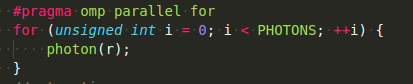
\includegraphics[width=2in]{imagenes/opt_omp_lin_1.png} \pause
        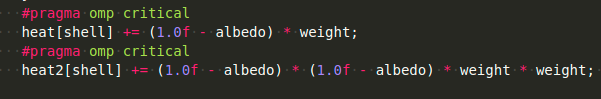
\includegraphics[width=2in]{imagenes/opt_omp_lin_2.png}
    \end{frame}

    \begin{frame}
        \frametitle{Paralelizando el tinymc no vectorizado}
        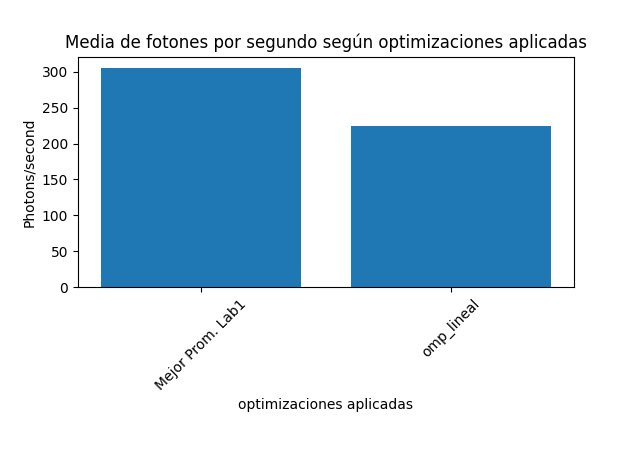
\includegraphics[width=4in]{imagenes/comp_prom_1.png}
    \end{frame}

    \begin{frame}
        \frametitle{Paralelizando el tinymc no vectorizado}
        Principales Problemas
        \begin{itemize}
            \item False sharing
            \item scheduling no dinámico
        \end{itemize}
    \end{frame}

    \begin{frame}
        \frametitle{Paralelizando el tinymc no vectorizado}
        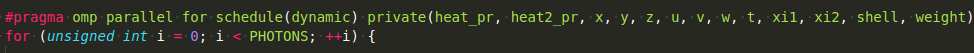
\includegraphics[width=4in]{imagenes/opt_omp_lin_3.png}

    \end{frame}

    \begin{frame}
        \frametitle{Paralelizando el tinymc no vectorizado}

        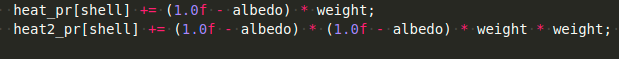
\includegraphics[width=3in]{imagenes/opt_omp_lin_4.png} \pause
        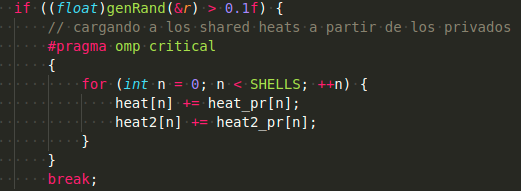
\includegraphics[width=2in]{imagenes/opt_omp_lin_5.png}

    \end{frame}

    \begin{frame}
        \frametitle{Paralelizando el tinymc no vectorizado}
        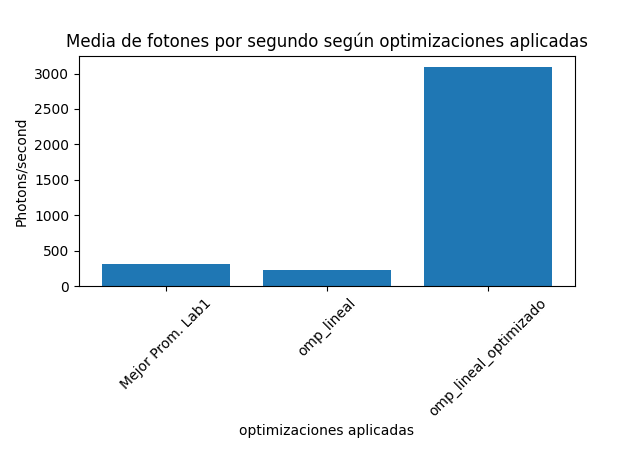
\includegraphics[width=4in]{imagenes/comp_prom_2.png}
    \end{frame}


\end{document}